\section*{4. Expectation}\label{expectation}

\subsection*{4.1 Expectation of a Random
Variable}\label{expectation-of-a-random-variable}
The \textbf{expected value}, \textbf{mean} or \textbf{first moment} of
\(X\) is defined to be
\[
\EXP(X) = \int x \; dF(x) = \begin{cases}
\sum_x x f(x) &\text{if } X \text{ is discrete} \\
\int x f(x)\; dx &\text{if } X \text{ is continuous}
\end{cases}
\]
assuming that the sum (or integral) is well-defined. We use the
following notation to denote the expected value of \(X\):
\[
\EXP(X) = \EXP X = \int x\; dF(x) = \mu = \mu_X
\]
The expectation is a one-number summary of the distribution. Think of
\(\EXP(X)\) as the average value you'd obtain if you computed the
numeric average \(n^{-1} \sum_{i=1}^{n} X_{i}\) for a large number of IID
draws \(X_{1}, \dots, X_{n}\). The fact that
\(\EXP(X) \approx n^{-1} \sum_{i=1}^{n} X_{i}\) is a Theorem called
the law of large numbers which we will discuss later. We use
\(\int x \; dF(x)\) as a convenient unifying notation between the
discrete case \(\sum_x x f(x)\) and the continuous case
\(\int x f(x) \; dx\) but you should be aware that \(\int x \; dF(x)\)
has a precise meaning discussed in real analysis courses.
To ensure that \(\EXP(X)\) is well defined, we say that
\(\EXP(X)\) exists if \(\int_x |x| \; dF_X(x) < \infty\).
Otherwise we say that the expectation does not exist. From now on,
wheneverwe discuss expectations, we implicitly assume they exist.

\textbf{Theorem 4.6 (The rule of the lazy statician)}. Let \(Y = r(X)\).
Then
\[
\EXP(Y) = \EXP(r(X)) = \int r(x) \; dF_X(x)
\]
As a special case, let \(A\) be an event and let \(r(x) = I_A(x)\),
where \(I_A(x) = 1\) if \(x \in A\) and \(I_A(x) = 0\) otherwise. Then
\[
\EXP(I_A(X)) = \int I_A(x) f_X(x) dx = \int_A f_X(x) dx = \PROB(X \in A)
\]
In other words, probability is a special case of expectation.
Functions of several variables are handled in a similar way. If
\(Z = r(X, Y)\) then
\[
\EXP(Z) = \EXP(r(X, Y)) = \int \int r(x, y) \; dF(x, y)
\]
The \textbf{\(k\)-th moment} of \(X\) is defined to be
\(\EXP(X^{k})\), assuming that \(\EXP(|X|^{k}) < \infty\). We
shall rarely make much use of moments beyond \(k = 2\).

\subsection*{4.2 Properties of
Expectations}\label{properties-of-expectations}

\textbf{Theorem 4.10}. If \(X_{1}, \dots, X_{n}\) are random variables and
\(a_{1}, \dots, a_{n}\) are constants, then
\[
\EXP\left( \sum_{i} a_{i} X_{i} \right) = \sum_{i} a_{i} \EXP(X_{i})
\]

\textbf{Theorem 4.12}. Let \(X_{1}, \dots, X_{n}\) be independent random
variables. Then,
\[
\EXP\left(\prod_{i} X_{i} \right) = \prod_{i} \EXP(X_{i})
\]
Notice that the summation rule does not require independence but the
product does.

\subsection*{4.3 Variance and
Covariance}\label{variance:covariance}
Let \(X\) be a random variable with mean \(\mu\). The \textbf{variance}
of \(X\) -- denoted by \(\sigma^{2}\) or \(\sigma_X^{2}\) or
\(\VAR(X)\) or \(\VAR X\) -- is defined by
\[
\sigma^{2} = \EXP(X - \mu)^{2} = \int (x - \mu)^{2}\; dF(x)
\]
assuming this expectation exists. The \textbf{standard deviation} is
\(\SD(X) = \sqrt{\VAR(X)}\) and is also denoted by
\(\sigma\) and \(\sigma_X\).

\textbf{Theorem 4.14}. Assuming the variance is well defined, it has the
following properties:
\begin{enumerate}[label={\arabic*.}]
\item
  \(\VAR(X) = \EXP(X^{2}) - \EXP(X)^{2}\)
\item
  If \(a\) and \(b\) are constants then
  \(\VAR(aX + b) = a^{2} \VAR(X)\)
\item
  If \(X_{1}, \dots, X_{n}\) are independent and \(a_{1}, \dots, a_{n}\) are
  constants then
  \[
\VAR\left( \sum_{i=1}^{n} a_{i}X_{i} \right) = \sum_{i=1}^{n} a_{i}^{2} \VAR(X_{i})
\]
\end{enumerate}
If \(X_{1}, \dots, X_{n}\) are random variables then we define the
\textbf{sample mean} to be
\[
\bar{X}_{n} = \frac{1}{n} \sum_{i=1}^{n} X_{i} 
\]
and the \textbf{sample variance} to be
\[
S_{n}^{2} = \frac{1}{n - 1} \sum_{i=1}^{n} \left(X_{i} - \bar{X}_{n}\right)^{2}
\]

\textbf{Theorem 4.16}. Let \(X_{1}, \dots, X_{n}\) be IID and let
\(\mu = \EXP(X_{i})\), \(\sigma^{2} = \VAR(X_{i})\). Then
\[
\EXP\left(\bar{X}_{n}\right) = \mu,
\quad
\VAR\left(\bar{X}_{n}\right) = \frac{\sigma^{2}}{n},
\quad \text{and} \quad
\EXP\left(S_{n}^{2}\right) = \sigma^{2}
\]
If \(X\) and \(Y\) are random variables, then the covariance and
correlation between \(X\) and \(Y\) measure how strong the linear
relationship between \(X\) and \(Y\) is.
Let \(X\) and \(Y\) be random variables with means \(\mu_X\) and
\(\mu_Y\) and standard deviation \(\sigma_X\) and \(\sigma_Y\). Define
the \textbf{covariance} between \(X\) and \(Y\) by
\[
\COV(X, Y) = \EXP[(X - \mu_X)(Y - \mu_Y)]
\]
and the \textbf{correlation} by
\[
\rho = \rho_{X, Y} = \rho(X, Y) = \frac{\COV(X, Y)}{\sigma_X \sigma_Y}
\]

\textbf{Theorem 4.18}. The covariance satisfies:
\[
\COV(X, Y) = \EXP(XY) - \EXP(X) \EXP(Y)
\]
The correlation satisfies:
\[
-1 \leq \rho(X, Y) \leq 1
\]
If \(Y = a + bX\) for some constants \(a\) and \(b\) then
\(\rho(X, Y) = 1\) if \(b > 0\) and \(\rho(X, Y) = -1\) if \(b < 0\). If
\(X\) and \(Y\) are independent, then \(\COV(X, Y) = \rho = 0\).
The converse is not true in general.

\textbf{Theorem 4.19}.
\[
\VAR(X + Y) = \VAR(X) + \VAR(Y) + 2 \COV(X, Y)
\quad \text{ and } \quad
\VAR(X - Y) = \VAR(X) + \VAR(Y) - 2 \COV(X, Y)
\]
More generally, for random variables \(X_{1}, \dots, X_{n}\),
\[
\VAR\left( \sum_{i} a_{i} X_{i} \right) = \sum_{i} a_{i}^{2} \VAR(X_{i}) + 2 \sum \sum_{i < j} a_{i} a_{j} \COV(X_{i}, X_{j})
\]

\subsection*{4.4 Expectation and Variance of Important Random
Variables}\label{expectation-and-variance-of-important-random-variables}
\[
\begin{array}{lll}
\text{Distribution} & \text{Mean} & \text{Variance}\\
\hline
\text{Point mass at } p      & a             & 0                \\
\text{Bernoulli}(p)          & p             & p(1-p)           \\
\text{Binomial}(n, p)        & np            & np(1-p)          \\
\text{Geometric}(p)          & 1/p           & (1 - p)/p^{2}    \\
\text{Poisson}(\lambda)      & \lambda       & \lambda          \\
\text{Uniform}(a, b)         & (a + b) / 2   & (b - a)^{2} / 12 \\
\text{Normal}(\mu, \sigma^{2}) & \mu           & \sigma^{2}     \\
\text{Exponential}(\beta)    & \beta         & \beta^{2}        \\
\text{Gamma}(\alpha, \beta)  & \alpha \beta  & \alpha \beta^{2} \\
\text{Beta}(\alpha, \beta)   & \alpha / (\alpha + \beta) & \alpha \beta / ((\alpha + \beta)^{2} (\alpha + \beta + 1)) \\
t_\nu                        & 0 \text{ (if } \nu > 1 \text{)} & \nu / (\nu - 2) \text{ (if } \nu > 2 \text{)} \\
\chi^{2}_{p}                     & p             & 2p           \\
\text{Multinomial}(n, p)     & np            & \text{see below} \\
\text{Multivariate Nornal}(\mu, \Sigma) & \mu & \Sigma \\
\end{array}
\]
The last two entries in the table are multivariate models which involve
a random vector \(X\) of the form
\[
X = \begin{pmatrix} X_{1} \\ \vdots \\ X_{k} \end{pmatrix}
\]
The mean of a random vector \(X\) is defined by
\[
\mu = \begin{pmatrix} \mu_{1} \\ \vdots \\ \mu_{k} \end{pmatrix} = \begin{pmatrix} \EXP(X_{1}) \\ \vdots \\ \EXP(X_{k}) \end{pmatrix}
\]
The \textbf{Variance-Covariance Matrix} \(\Sigma\) is defined to be
\[
\Sigma = \begin{pmatrix}
\VAR(X_{1}) & \COV(X_{1}, X_{2}) & \cdots & \COV(X_{1}, X_{k}) \\
\COV(X_{2}, X_{1}) & \VAR(X_{2}) & \cdots & \COV(X_{2}, X_{k}) \\
\vdots & \vdots & \ddots & \vdots \\
\COV(X_{k}, X_{1}) & \COV(X_{k}, X_{2}) & \cdots & \VAR(X_{k})
\end{pmatrix}
\]
If \(X \sim \text{Multinomial}(n, p)\) then
\[
\EXP(X) = np = n(p_{1}, \dots, p_{k})
\quad \text{and} \quad
\VAR(X) = \begin{pmatrix}
np_{1}(1 - p_{1}) & -np_{1}p_{2} & \cdots & -np_{1}p_{k} \\
-np_{2}p_{1} & np_{2}(1 - p_{2}) & \cdots & -np_{2}p_{k} \\
\vdots & \vdots & \ddots & \vdots \\
-np_{k}p_{1} & -np_{k}p_{2} & \cdots & np_{k}(1 - p_{k})
\end{pmatrix}
\]
To see this:
\begin{itemize}[tightlist]
\item
  Note that the marginal distribution of any one component is
  \(X_{i} \sim \text{Binomial}(n, p_{i})\), so \(\EXP(X_{i}) = np_{i}\)
  and \(\VAR(X_{i}) = np_{i}(1 - p_{i})\).\\
\item
  Note that, for \(i \neq j\),
  \(X_{i} + X_{j} \sim \text{Binomial}(n, p_{i} + p_{j})\), so
  \(\VAR(X_{i} + X_{j}) = n(p_{i} + p_{j})(1 - (p_{i} + p_{j}))\).
\item
  Using the formula for the covariance of a sum, for \(i \neq j\),
\end{itemize}
\[
\VAR(X_{i} + X_{j}) = \VAR(X_{i}) + \VAR(X_{j}) + 2 \COV(X_{i}, X_{j}) =  np_{i}(1 - p_{i}) + np_{j}(1 - p_{j}) + 2 \COV(X_{i}, X_{j})
\]
Equating the last two formulas we get a formula for the covariance,
\(\COV(X_{i}, X_{j}) = -np_{i}p_{j}\).
Finally, here is a lemma that can be useful for finding means and
variances of linear combinations of multivariate random vectors.
\textbf{Lemma 4.20}. If \(a\) is a vector and \(X\) is a random vector
with mean \(\mu\) and variance \(\Sigma\) then
\[
\EXP(a^T X) = a^T \mu
\quad \text{and} \quad
\VAR(a^T X) = a^T \Sigma a
\]
If \(A\) is a matrix then
\[
\EXP(A X) = A \mu
\quad \text{and} \quad
\VAR(AX) = A \Sigma A^T
\]

\subsection*{4.5 Conditional
Expectation}\label{conditional-expectation}
The conditional expectation of \(X\) given \(Y = y\) is
\[
\EXP(X | Y = y) = \begin{cases}
\sum x f_{X | Y}(x | y) &\text{ discrete case} \\
\int x f_{X | Y}(x | y) dy &\text{ continuous case}
\end{cases}
\]
If \(r\) is a function of \(x\) and \(y\) then
\[
\EXP(r(X, Y) | Y = y) = \begin{cases}
\sum r(x, y) f_{X | Y}(x | y) &\text{ discrete case} \\
\int r(x, y) f_{X | Y}(x | y) dy &\text{ continuous case}
\end{cases}
\]
While \(\EXP(X)\) is a number, \(\EXP(X | Y = y)\) is a
function of \(y\). Before we observe \(Y\), we do not know the value of
\(\EXP(X | Y = y)\) so it is a random variable which we denote
\(\EXP(X | Y)\). In other words, \(\EXP(X | Y)\) is the
random variable whose value is \(\EXP(X | Y = y)\) when \(Y\) is
observed as \(y\). Similarly, \(\EXP(r(X, Y) | Y)\) is the random
variable whose value is \(\EXP(r(X, Y) | Y = y)\) when \(Y\) is
observed as \(y\).

\textbf{Theorem 4.23 (The rule of iterated expectations)}. For random
variables \(X\) and \(Y\), assuming the expectations exist, we have that
\[
\EXP[\EXP(Y | X)] = \EXP(Y)
\quad \text{and} \quad
\EXP[\EXP(X | Y)] = \EXP(X)
\]
More generally, for any function \(r(x, y)\) we have
\[
\EXP[\EXP(r(X, Y) | X)] = \EXP(r(X, Y))
\quad \text{and} \quad
\EXP[\EXP(r(X, Y) | Y)] = \EXP(r(X, Y))
\]
\textbf{Proof}. We will prove the first equation.
\begin{align*}
\EXP[\EXP(Y | X)] &= \int \EXP(Y | X = x) f_X(x) dx = \int \int y f(y | x) dy f(x) dx \\
&= \int \int y f(y|x) f(x) dx dy = \int \int y f(x, y) dx dy = \EXP(Y)
\end{align*}
The \textbf{conditional variance} is defined as
\[
\VAR(Y | X = x) = \int (y - \mu(x))^{2} f(y | x) dx
\]
where \(\mu(x) = \EXP(Y | X = x)\).

\textbf{Theorem 4.26}. For random variables \(X\) and \(Y\),
\[
\VAR(Y) = \EXP\VAR(Y | X) + \VAR \EXP (Y | X)
\]

\subsection*{4.6 Technical Appendix}
\paragraph{4.6.1 Expectation as an
Integral}\label{expectation-as-an-integral}
The integral of a measurable function \(r(x)\) is defined as follows.
First suppose that \(r\) is simple, meaning that it takes finitely many
values \(a_{1}, \dots, a_{k}\) over a partition \(A_{1}, \dots, A_{k}\). Then
\(\int r(x) dF(x) = \sum_{i=1}^{k} a_{i} \PROB(r(X) \in A_{i})\). The
integral of a positive measurable function \(r\) is defined by
\(\int r(x) dF(x) = \lim_{i} \int r_{i}(x) dF(x)\), where \(r_{i}\) is a
sequence of simple functions such that \(r_{i}(x) \leq r(x)\) and
\(r_{i}(x) \rightarrow r(x)\) as \(i \rightarrow \infty\). This does not
depend on the particular sequence. The integral of a measurable function
\(r\) is defined to be
\(\int r(x) dF(x) = \int r^+(x) dF(x) - \int r^-(x) dF(x)\) assuming
both integrals are finite, where \(r^+(x) = \max \{ r(x), 0 \}\) and
\(r^-(x) = \min\{ r(x), 0 \}\).
\paragraph{4.6.2 Moment Generating
Functions}\label{moment-generating-functions}
The \textbf{moment generating function (mgf)} or \textbf{Laplace
transform} of \(X\) is defined by
\[
\psi_X(t) = \EXP(e^{tX}) = \int e^{tx} dF(x)
\]
where \(t\) varies over the real numbers.
In what follows, we assume the mgf is well defined for all \(t\) in
small neighborhood of 0. A related function is the characteristic
function, defined by \(\EXP(e^{itX})\) where \(i = \sqrt{-1}\).
This function is always defined for all \(t\). The mgf is useful for
several reasons. First, it helps us compute the moments of a
distribution. Second, it helps us find the distribution of sums of
random variables. Third, it is used to prove the central limit Theorem.
When the mgf is well defined, it can be shown that we can interchange
the operations of differentiation and ``taking expectation''. This leads
to
\[
\psi'(0) = \left[ \frac{d}{dt} \EXP e^{tX} \right]_{t = 0} = \EXP \left[ \frac{d}{dt} e^{tX} \right]_{t = 0}
= \EXP[X e^{tX}]_{t = 0} = \EXP(X)
\]
By taking further derivatives we conclude that
\(\psi^{(k)}(0) = \EXP(X^{k})\). This gives us a method for
computing the moments of a distribution.
\textbf{Lemma 4.30}. Properties of the mgf.
\begin{enumerate}[tightlist,label={\arabic*.}]
\item
  If \(Y = aX + b\) then \(\psi_{Y(t)} = e^{bt} \psi_{X(at)}\)
\item
  if \(X_{1}, \dots, X_{n}\) are independent and \(Y = \sum_{i} X_{i}\) then
  \(\psi_Y(t) = \prod_{i} \psi_{i}(t)\), where \(\psi_{i}\) is the mgf of
  \(X_{i}\).
\end{enumerate}

\textbf{Theorem 4.32}. Let \(X\) and \(Y\) be random variables. If
\(\psi_X(t) = \psi_Y(t)\) for all \(t\) in an open interval around 0,
then \(X \overset{d}= Y\).
\textbf{Moment Generating Function for Some Common Distributions}
\[
\begin{array}{ll}
\text{Distribution} & \text{mgf} \\
\hline
\text{Bernoulli}(p)   & pe^t + (1 - p)         \\
\text{Binomial}(n, p) & (pe^t + (1 - p))^{n}     \\
\text{Poisson}(\lambda) & e^{\lambda(e^t - 1)} \\
\text{Normal}(\mu, \sigma^{2}) & \exp\left\{\mu t + \frac{\sigma^{2} t^{2}}{2} \right\} \\
\text{Gamma}(\alpha, \beta) & \left( \frac{\beta}{\beta - t} \right)^\alpha \text{ for } t < \beta
\end{array}
\]

\subsection*{4.7 Exercises}

\textbf{Exercise 4.7.1}. Suppose we play a game where we start with
\(c\) dollars. On each play of the game you either double your money or
half your money, with equal probability. What is your expected fortune
after \(n\) trials?

\textbf{Solution}. Let the random variables \(X_{i}\) be the fortune after
the \(i\)-th trial, \(X_{0} = c\) always taking the value \(c\). Then:
\[
\EXP[X_{i + 1} | X_{i} = x] = 2x \cdot \frac{1}{2} + \frac{x}{2} \cdot \frac{1}{2} = \frac{5}{4}x
\]
Taking the expectation on \(X_{i}\) on both sides (i.e.~integrating over
\(F_{X_{i}}(x)\)),
\[
\EXP(\EXP[X_{i + 1} | X_{i} = x]) = \frac{5}{4} \EXP(X_{i}) \Longrightarrow \EXP(X_{i+1}) = \frac{5}{4}  \EXP(X_{i})
\]
Therefore, by induction,
\[
\EXP(X_{n}) = \left(\frac{5}{4}\right)^{n} c
\]
Note that this is \textbf{not} a martingale, as in the traditional
double-or-nothing formulation -- the expected value goes up at each
iteration.

\textbf{Exercise 4.7.2}. Show that \(\VAR(X) = 0\) if and only if
there is a constant \(c\) such that \(\PROB(X = c) = 1\).

\textbf{Solution}. We have
\(\VAR(X) = \EXP[(X - \EXP(X))^{2}]\):
\[
\VAR(X) = \int (x - \mu_X)^{2} dF_X(x)
\]
Since \((x - \mu_X)^{2} \geq 0\), in order for the variance to be 0 we
must have the integrand be zero with probability 1,
i.e.~\(\PROB(X = \mu_X) = 1\).

\textbf{Exercise 4.7.3}. Let
\(X_{1}, \dots, X_{n} \sim \text{Uniform}(0, 1)\) and let
\(Y_{n} = \max \{ X_{1}, \dots, X_{n} \}\). Find \(\EXP(Y_{n})\).

\textbf{Solution}. The CDF of \(Y_{n}\), for \(0 \leq y \leq 1\), is:
\[
F_{Y_{n}}(y) = \PROB(Y_{n} \leq y) = \prod_{i=1}^{n} \PROB(X_{i} \leq y) = y^{n}
\]
so its PDF is \(f_{Y_{n}}(y) = F'_{Y_{n}}(y) = n y^{n-1}\) for
\(0 \leq y \leq 1\).
The expected value of \(Y_{n}\) then is
\[
\EXP(Y_{n}) = \int_{0}^{1} y f_{Y_{n}}(y) dy = \int_{0}^{1} n y^{n} dy = \frac{n}{n+1}
\]

\textbf{Exercise 4.7.4}. A particle starts at the origin of the real
line and moves along the line in jumps of one unit. For each jump the
probability is \(p\) that the particle will move one unit to the left
and the probability is \(1 - p\) that the particle will jump one unit to
the right. Let \(X_{n}\) be the position of the particle after \(n\)
units. Find \(\EXP(X_{n})\) and \(\VAR(X_{n})\). (This is known
as a random walk.)

\textbf{Solution}.
We can define \(X_{n} = \sum_{i=1}^{n} (1 - 2Y_{i})\), where
\(Y_{i} \sim \text{Bernoulli}(p)\) and the \(Y_{i}\)s are independent
random variables representing the direction of each jump.
We then have:
\[
\EXP(X_{n}) = \sum_{i=1}^{n} \EXP(1 - 2Y_{i}) = \sum_{i=1}^{n} (1 - 2p) = n(1 - 2p)
\]
and
\[
\VAR(X_{n}) = \sum_{i=1}^{n} \VAR(1 - 2Y_{i}) \sum_{i=1}^{n} 4\VAR(Y_{i}) = 4np(1 - p)
\]

\textbf{Exercise 4.7.5}. A fair coin is tossed until a head is obtained.
What is the expected number of tosses that will be required?

\textbf{Solution}. The number of tosses follows a geometric
distribution, \(X \sim \text{Geom}(p)\), where \(p\) is the probability
of heads. Deduce its expected value, rather than use it as a known
fact (\(\EXP(X) = 1/p\)). The PDF is
\[
f_X(k) = p (1 - p)^{k - 1}, \quad k > 0
\]
The expected value for \(X\) is
\begin{align*}
\EXP(X) &= \sum_{k=1}^{\infty} k p (1 - p)^{k - 1}  \\
&= \sum_{k=1}^{\infty} p(1-p)^{k-1} + \sum_{k=2}^{\infty} (k - 1) p(1-p)^{k - 1} \\
&= p \left( 1 + (1 - p) + (1 - p)^{2} + \dots \right) + \sum_{k=1}^{\infty} k p(1-p)^{k} \\
&= p \left(\frac{1}{1 - (1 - p)}\right) + (1 - p) \sum_{k=1}^{\infty} k p(1-p)^{k - 1} \\
&= 1 + (1 - p) \EXP(X)
\end{align*}
from where we get \(\EXP(X) = 1 / p\).

\textbf{Exercise 4.7.6}. Prove Theorem 4.6 for discrete random
variables.
Let \(Y = r(X)\). Then
\[
\EXP(Y) = \EXP(r(X)) = \int r(x) \; dF_X(x)
\]

\textbf{Solution}. The result is immediate from the definition of
expectation:
\[
Y(\omega) = r(X(\omega)) = r(x) \quad \forall \omega : X(\omega) = x
\]
and so
\[
\EXP(Y) = \int r(x) dF_x(x)
\]

\textbf{Exercise 4.7.7}. Let \(X\) be a continuous random variable with
CDF \(F\). Suppose that \(\PROB(X > 0) = 1\) and that
\(\EXP(X)\) exists. Show that
\(\EXP(X) = \int_{0}^{\infty} \PROB(X > x) dx\).
Hint: Consider integrating by parts. The following fact is helpful: if
\(\EXP(X)\) exists then
\(\lim_{x \rightarrow +\infty} x | 1 - F(x) | = 0\).

\textbf{Solution}. Prove the following, slightly more general,
lemma.
Lemma: For every continuous random variable \(X\),
\[
\EXP(X) = \int_{0}^{\infty} (1 - F_X(y)) dy - \int_{-\infty}^{0} F_X(y) dy
\]
Proof:
\begin{align*}
\EXP(X) &= \int_{-\infty}^{\infty} x f_X(x) dx \\
&= \int_{-\infty}^{0} \int_x^{0} -f_X(x) dy dx + \int_{0}^{\infty} \int_{0}^x f_X(x) dy dx \\
&= -\int_{-\infty}^{0} \int_{-\infty}^y f_X(x) dx dy + \int_{0}^{\infty} \int_y^{\infty} f_X(x) dx dy \\
&= -\int_{\infty}^{0} \PROB(X \leq y) dy + \int_{0}^{\infty} \PROB(X \geq y) dy \\
&= \int_{0}^{\infty} (1 - F_X(y)) dy - \int_{-\infty}^{0} F_X(y) dy
\end{align*}
The result follows by imposing \(\PROB(X > 0) = 1\), which implies
\(\int_{-\infty}^{0} F_X(y) dy = 0\).

\textbf{Exercise 4.7.8}. Prove Theorem 4.16.
Let \(X_{1}, \dots, X_{n}\) be IID and let \(\mu = \EXP(X_{i})\),
\(\sigma^{2} = \VAR(X_{i})\). Then
\[
\EXP\left(\bar{X}_{n}\right) = \mu,
\quad
\VAR\left(\bar{X}_{n}\right) = \frac{\sigma^{2}}{n},
\quad \text{and} \quad
\EXP\left(S_{n}^{2}\right) = \sigma^{2}
\]

\textbf{Solution}.
For the expected value of sample mean:
\[
\EXP\left(\bar{X}_{n}\right) 
= \EXP\left( \frac{1}{n} \sum_{i=1}^{n} X_{i} \right)
= \frac{1}{n} \sum_{i=1}^{n} \EXP(X_{i})
= \frac{1}{n} n\mu = \mu
\]
For the variance of sample mean:
\[
\VAR\left(\bar{X}_{n}\right) 
= \VAR\left( \frac{1}{n} \sum_{i=1}^{n} X_{i} \right)
= \frac{1}{n^{2}} \sum_{i=1}^{n} \VAR(X_{i})
= \frac{1}{n^{2}} n \sigma^{2} = \frac{\sigma^{2}}{n}
\]
For the expected value of sample variance:
\begin{align*}
\EXP(S_{n}^{2}) &= \EXP\left(\frac{1}{n - 1} \sum_{i=1}^{n} \left(X_{i} - \bar{X}_{n}\right)^{2} \right) \\
&= \frac{1}{n - 1} \EXP \left( \sum_{i=1}^{n} \left(X_{i} - \bar{X}_{n}\right)^{2} \right) \\
&= \frac{1}{n - 1} \EXP \left( \sum_{i=1}^{n} X_{i}^{2} - 2 X_{i} \bar{X}_{n} + \bar{X}_{n}^{2} \right) \\
&= \frac{1}{n - 1} \EXP \left( \sum_{i=1}^{n} X_{i}^{2} - 2 \bar{X}_{n} \sum_{i=1}^{n} X_{i} + n \bar{X}_{n}^{2} \right) \\
&= \frac{1}{n - 1} \EXP \left( \sum_{i=1}^{n} X_{i}^{2} - 2 \bar{X}_{n} \cdot n \bar{X}_{n}  + n \bar{X}_{n}^{2} \right) \\
&= \frac{1}{n - 1} \EXP \left( \sum_{i=1}^{n} X_{i}^{2} - n \bar{X}_{n}^{2} \right) \\
&= \frac{1}{n - 1} \left( \sum_{i=1}^{n}  \EXP(X_{i}^{2}) - n \EXP\left( \bar{X}_{n}^{2} \right) \right) \\
&= \frac{1}{n - 1} \left( \sum_{i=1}^{n} \left(\VAR(X_{i}) + \EXP(X_{i})^{2} \right) - n \left(\VAR\left( \bar{X}_{n} \right) + \EXP\left(\bar{X}_{n}\right)^{2} \right)\right) \\
&= \frac{1}{n -1} \left( n \left( \sigma^{2} + \mu^{2}\right) - n \left(\frac{\sigma^{2}}{n} + \mu^{2} \right) \right) \\
&= \sigma^{2}
\end{align*}

\textbf{Exercise 4.7.9 (Computer Experiment)}. Let \(X_{1}, \dots, X_{n}\)
be \(N(0, 1)\) random variables and let
\(\bar{X}_{n} = n^{-1} \sum_{i=1}^{n} X_{i}\). Plot \(\bar{X}_{n}\)
versus \(n\) for \(n = 1, \dots, 10,000\). Repeat for
\(X_{1}, \dots, X_{n} \sim \text{Cauchy}\). Explain why there is such a
difference.

\begin{python}
import numpy as np
from scipy.stats import norm, cauchy
np.random.seed(0)
N = 10000
X = norm.rvs(size=N)
Y = cauchy.rvs(size = N)
\end{python}

\begin{python}
import matplotlib.pyplot as plt
nn = np.arange(1, N + 1)
plt.figure(figsize=(12, 8))
ax = plt.subplot(2, 1, 1)
ax.plot(nn, np.cumsum(X) / nn)
ax.set_title('N(0, 1)')
ax.set_xlabel('n')
ax.set_ylabel(r'$\bar{X}_{n}$')
ax = plt.subplot(2, 1, 2)
ax.plot(nn, np.cumsum(Y) / nn)
ax.set_title('Cauchy')
ax.set_xlabel('n')
ax.set_ylabel(r'$\bar{X}_{n}$')
plt.tight_layout()
plt.show()
\end{python}

\begin{figure}[H]
\centering
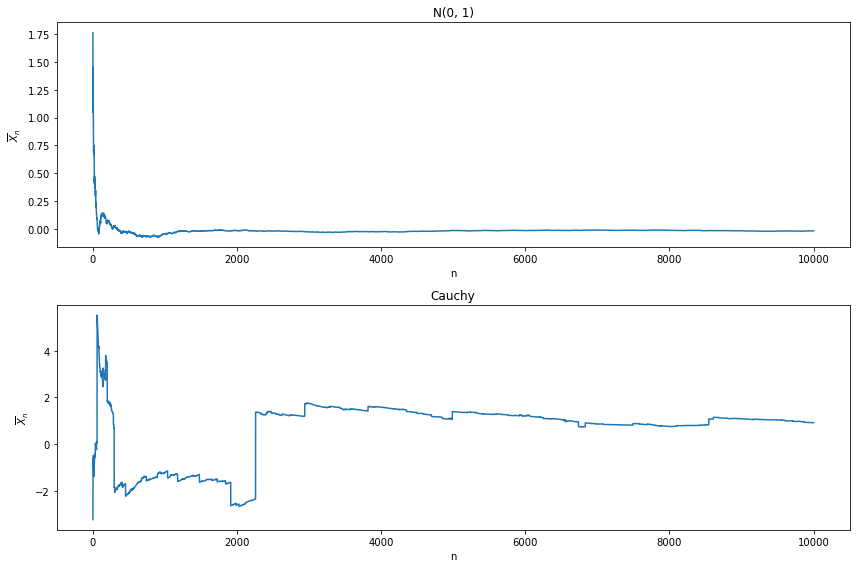
\includegraphics{Figure-04-01}
\end{figure}

The mean on the Cauchy distribution is famously undefined:
\(\bar{X}_ n\) is not going to converge.

\textbf{Exercise 4.7.10}. Let \(X \sim N(0, 1)\) and let \(Y = e^X\).
Find \(\EXP(Y)\) and \(\VAR(Y)\).

\textbf{Solution}.
The CDF of \(Y\) is, for \(y > 0\):
\[
F_Y(y) = \PROB(Y \leq y) = \PROB(X \leq \log y) = \Phi(\log y)
\]
and so the PDF is
\[
f_Y(y) = F'_Y(y) = \frac{d}{dy} \Phi(\log y) = \frac{d \Phi(\log y)}{d \log y} \frac{d \log y}{dy} = \frac{\phi(\log y)}{y}
\]
The expected value is
\[
\EXP(Y) = \int y f_Y(y) dy = \int_{0}^{\infty} y \frac{\phi(\log y)}{y} dy = \int_{0}^{\infty} \phi(\log y)\; dy = \sqrt{e}
\]
The expected value of \(Y^{2}\) is
\[
\EXP(Y^{2}) = \int y^{2} f_Y(y) dy = \int_{0}^{\infty} y^{2} \frac{\phi(\log y)}{y} dy = \int_{0}^{\infty} y \phi(\log y)\; dy = e^{2}
\]
and so the variance is
\[
\VAR(Y) = \EXP(Y^{2}) - \EXP(Y)^{2} = e(e - 1)
\]

\textbf{Exercise 4.7.11 (Computer Experiment: Simulating the Stock
Market)}. Let \(Y_{1}, Y_{2}, \dots\) be independent random variables such
that \(\PROB(Y_{i} = 1) = \PROB(Y_{i} = -1) = 1/2\). Let
\(X_{n} = \sum_{i=1}^{n} Y_{i}\). Think of \(Y_{i} = 1\) as ``the stock price
increased by one dollar'' \(Y_{i} = -1\) as ``the stock price decreased by
one dollar'' and \(X_{n}\) as the value of the stock on day \(n\).
\textbf{(a)} Find \(\EXP(X_{n})\) and \(\VAR(X_{n})\).
\textbf{(b)} Simulate \(X_{n}\) and plot \(X_{n}\) versus \(n\) for
\(n = 1, 2, \dots, 10,000\). Repeat the whole simulation several times.
Notice two things. First, it is easy to ``see'' patterns in the sequence
even though it is random. Second, you will find that the runs look very
different even though they were generated the same way. How do the
calculations in (a) explain the second observation?

\textbf{Solution}.
\textbf{(a)} We have:
\[
\EXP(X_{n}) = \EXP\left( \sum_{i=1}^{n} Y_{i} \right) = \sum_{i=1}^{n} \EXP(Y_{i}) = 0
\]
and
\begin{align*}
\EXP(X_{n}^{2}) &= \EXP\left( \left( \sum_{i=1}^{n} Y_{i} \right)^{2} \right) \\
&= \EXP\left( \sum_{i=1}^{n} Y_{i}^{2} + \sum_{i=1}^{n} \sum_{j = 1, j \neq i}^{n} Y_{i} Y_{j} \right) \\
&= \sum_{i=1}^{n} \EXP(Y_{i}^{2}) + \sum_{i=1}^{n} \sum_{j = 1, j \neq i}^{n} \EXP(Y_{i} Y_{j}) \\
&= \sum_{i=1}^{n} 1 + \sum_{i=1}^{n} \sum_{j = 1, j \neq i}^{n} 0 \\
&= n
\end{align*}
so
\[
\VAR(X_{n}) = \EXP(X_{n}^{2}) - \EXP(X_{n})^{2} = n
\]
\textbf{(b)}

\begin{python}
import numpy as np
from scipy.stats import norm, bernoulli
N = 10000
B = 20
Y = 2 * bernoulli.rvs(p=1/2, loc=0, size=(B, N), random_state=0) - 1
X = np.cumsum(Y, axis=1)
\end{python}

\begin{python}
import matplotlib.pyplot as plt
plt.figure(figsize=(12, 8))
nn = np.arange(1, N + 1)
z = norm.ppf(0.975)
plt.plot(nn, z * np.sqrt(nn), color='red')
plt.plot(nn, -z * np.sqrt(nn), color='red')
plt.fill_between(nn, z * np.sqrt(nn), -z * np.sqrt(nn), color='red', alpha=0.05)
for b in range(B):
    plt.plot(nn, X[b])
    
plt.show()
\end{python}

\begin{figure}[H]
\centering
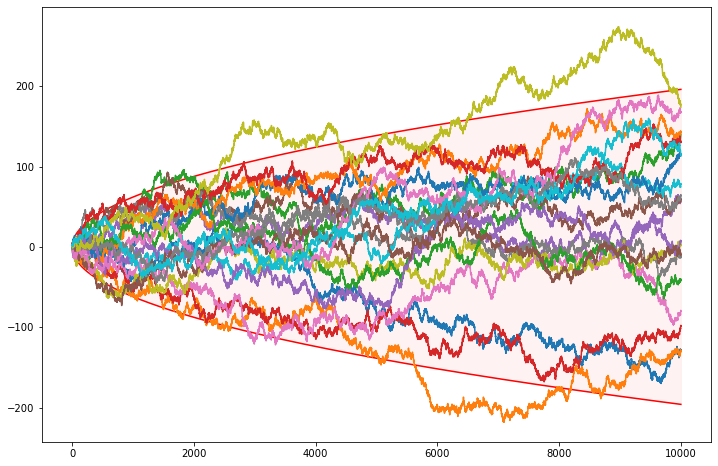
\includegraphics{Figure-04-02}
\end{figure}

The standard deviation is \(\sqrt{n}\) -- it scales up with the square
root of the ``time''. The plot above draws \(z_{\alpha / 2} \sqrt{n}\)
curves -- confidence bands for \(1 - \alpha = 95\%\) -- that contain
most of the randomly generated path.

\textbf{Exercise 4.7.12}. Prove the formulas given in the table at the
beginning of Section 4.4 for the Bernoulli, Poisson, Uniform,
Exponential, Gamma, and Beta. Here are some hints. For the mean of the
Poisson, use the fact that \(e^{a} = \sum_{x=0}^{a} a^x / x!\). To compute
the variance, first compute \(\EXP(X(X - 1))\). For the mean of
the Gamma, it will help to multiply and divide by
\(\Gamma(\alpha + 1) / \beta^{\alpha + 1}\) and use the fact that a
Gamma density integrates to 1. For the Beta, multiply and divide by
\(\Gamma(\alpha + 1) \Gamma(\beta) / \Gamma(\alpha + \beta + 1)\).

\textbf{Solution}.
We will do all expressions in the table instead (other than multinomial
and multivariate normal, where proofs are already provided in the book).
\textbf{Point mass at \(p\)}. Let \(X\) have a point mass at \(p\).
Then:
\begin{itemize}[tightlist]
\item
  \(\EXP(X) = p \cdot 1 = p\)
\item
  \(\EXP(X^{2}) = p^{2} \cdot 1 = p^{2}\)
\item
  \(\VAR(X) = \EXP(X^{2}) - \EXP(X)^{2} = p^{2} - p^{2} = 0\)
\end{itemize}
\textbf{Bernoulli}. Let \(X \sim \text{Bernoulli}(p)\). Then:
\begin{itemize}[tightlist]
\item
  \(\EXP(X) = 1 \cdot p + 0 \cdot (1 - p) = p \)
\item
  \(\EXP(X^{2}) = 1 \cdot p + 0 \cdot (1 - p) = p\)
\item
  \(\VAR(X^{2}) = \EXP(X^{2}) - \EXP(X)^{2} = p(1 - p)\)
\end{itemize}
\textbf{Binomial}. Let \(X \sim \text{Binomial}(n, p)\). Then
\(X = \sum_{i=1}^{n} Y_{i}\), where \(Y_{i} \sim \text{Bernoulli}(p)\) are IID
random variables.
\begin{itemize}[tightlist]
\item
  \(\EXP(X) = \EXP\left( \sum_{i=1}^{n} Y\_{i} \right)
  = \sum_{i=1}^{n} \EXP(Y\_{i}) = np\)
\item
  \(\VAR(X) = \VAR\left(\sum_{i=1}^{n} Y\_{i} \right)
  = \sum_{i=1}^{n} \VAR(Y\_{i}) = np(1-p)\)
\end{itemize}
\textbf{Geometric}. Let \(X \sim \text{Geometric}(p)\). Then:
\begin{align*}
\EXP(X) &= \sum_{k=1}^{\infty} k p (1 - p)^{k - 1}  \\
&= \sum_{k=1}^{\infty} p(1-p)^{k-1} + \sum_{k=2}^{\infty} (k - 1) p(1-p)^{k - 1} \\
&= p \left( 1 + (1 - p) + (1 - p)^{2} + \dots \right) + \sum_{k=1}^{\infty} k p(1-p)^{k} \\
&= p \left(\frac{1}{1 - (1 - p)}\right) + (1 - p) \sum_{k=1}^{\infty} k p(1-p)^{k - 1} \\
&= 1 + (1 - p) \EXP(X)
\end{align*}
Solving for the expectation, we get \(\EXP(X) = 1/p\).
We also have:
\begin{align*}
\EXP(X^{2}) &= \sum_{k=1}^{\infty} k^{2} p (1 - p)^{k - 1}  \\
&= \sum_{k=1}^{\infty} k p(1-p)^{k-1} + \sum_{k=2}^{\infty} (k^{2} - k) p(1-p)^{k - 1} \\
&= \EXP(X) + (1 - p) \sum_{k=1}^{\infty} (k^{2} + k) p(1-p)^{k - 1} \\
&= \EXP(X) + (1 - p) \EXP(X) + (1 - p) \sum_{k=1}^{\infty} k^{2} p(1-p)^{k-1} \\
&= \frac{2 - p}{p} + (1 - p) \EXP(X^{2})
\end{align*}
Solving for the expectation, we get \(\EXP(X^{2}) = (2 - p) / p^{2}\).
Finally,
\[
\VAR(X) = \EXP(X^{2}) - \EXP(X)^{2} = \frac{2 - p}{p^{2}} - \frac{1}{p^{2}} = \frac{1 - p}{p^{2}}
\]
\textbf{Poisson}. Let \(X \sim \text{Poisson}(\lambda)\). Then:
\begin{itemize}
\item
  \( \EXP(X) = \sum_{k=0}^{\infty} k
  \frac{\lambda^{k} e^{-\lambda}}{k!} = \lambda e^{-\lambda}
  \sum_{k=1}^{\infty} \frac{\lambda^{k - 1} }{(k - 1)!} =
  \lambda e^{-\lambda} \sum_{k=0}^{\infty} \frac{\lambda^{k}}{k!}
  = \lambda e^{-\lambda} e^{\lambda} = \lambda \)
\item
  \( \EXP(X^{2}) = \sum_{k=0}^{\infty}k^{2}
  \frac{\lambda^{k} e^{-\lambda}}{k!} = \lambda \sum_{k=1}^{\infty} k
  \frac{\lambda^{k-1} e^{-\lambda} }{(k-1)!} =
  \lambda \sum_{k=0}^{\infty} (k + 1)
  \frac{\lambda^{k} e^{-\lambda} }{k!} = \lambda \EXP(X + 1) =
  \lambda(\lambda + 1) \)
\item
  \( \VAR(X) = \EXP(X^{2}) - \EXP(X)^{2} =
  \lambda^{2} + \lambda - \lambda^{2} = \lambda \)
\end{itemize}
\textbf{Uniform}. Let \(X \sim \text{Uniform}(a, b)\). Then:
\begin{itemize}[tightlist]
\item
  \(\EXP(X) = \int_a^{b} x \frac{1}{b - a} dx = \frac{a + b}{2}\)
\item
  \(\EXP(X^{2}) = \int_a^{b} x^{2} \frac{1}{b - a} dx = \frac{a^{2} + ab + b}{3}\)
\item
  \(\VAR(X) = \EXP(X^{2}) - \EXP(X)^{2} = \frac{a^{2} + ab + b}{3} - \frac{a^{2} + 2ab + b^{2}}{4} = \frac{(b - a)^{2}}{12}\)
\end{itemize}
\textbf{Normal}. Let \(X \sim N(\mu, \sigma^{2})\). Converting into a
standard normal, we get \(Z = (X - \mu) / \sigma \sim N(0, 1)\). Then:
\begin{itemize}[tightlist]
\item
  $ \EXP(X) = \EXP(\sigma Z + \mu) = \sigma \EXP(Z) +
  \mu = \mu$
\item
  $ \VAR(X) = \VAR(\sigma Z + \mu) = \sigma^{2}
  \VAR(Z) = \sigma^{2}$
\end{itemize}
To prove that the expected value \(Z\) is 0, note that the PDF of \(Z\)
is even, \(\phi(z) = \phi(-z)\), so
\begin{align*}
\EXP(Z) 
  = \int_{-\infty}^{\infty} z \phi(z) dz 
& = \int_{-\infty}^{0} z \phi(z) dz + \int_{0}^{\infty} z \phi(z) dz 
\\
& = \int_{0}^{\infty} -z \phi(-z) dz + \int_{0}^{\infty} z \phi(z) dz 
\\
& = \int_{0}^{\infty} (-z + z)\phi(z) = 0 
\end{align*}
To prove that the variance of \(Z\) is 0, write out the integral
explicitly for the expectation of \(Z^{2}\),
\begin{align*}
\EXP(Z^{2}) 
& = \int_{-\infty}^{\infty} z^{2} \phi(z) dz 
  = \frac{1}{\sqrt{2 \pi}} \int_{-\infty}^{\infty} z^{2} e^{-z^{2}/2} dz
  = \left[ \Phi(z) - \frac{1}{\sqrt{2 \pi}}  z e^{-z^{2}/2} \right]_{-\infty}^{\infty} 
\\
& = \lim_{x \rightarrow +\infty} \Phi(x) - \lim_{x \rightarrow -\infty} \Phi(x) 
  = 1 - 0 
  = 1
\end{align*}
and so
\[
\VAR(Z) = \EXP(Z^{2}) - \EXP(Z)^{2} = 1 - 0 = 1
\]
\textbf{Exponential}. Let \(X \sim \text{Exponential}(\beta)\). Then:
\begin{itemize}[tightlist]
\item
  \( \EXP(X) = \int_{0}^{\infty} x \frac{1}{\beta} e^{-x / \beta} dx = \frac{1}{\beta} \int_{0}^{\infty} x e^{-x / \beta}
  dx = \frac{1}{\beta} \beta^{2} = \beta \)
\item
  \( \EXP(X^{2}) = \int_{0}^{\infty} x2
  \frac{1}{\beta} e^{-x / \beta} dx = \frac{1}{\beta}
  \int_{0}^{\infty} x2 e^{-x / \beta} dx =
  \frac{1}{\beta} 2\beta^{3} = 2 \beta^{2} \)
\item
  \( \VAR(X) = \EXP(X^{2}) - \EXP(X)^{2} =
  2\beta^{2} - \beta^{2} = \beta^{2} \)
\end{itemize}
\textbf{Gamma}. Let \(X \sim \text{Gamma}(\alpha, \beta)\). The PDF is
\[
f_X(x) = \frac{\beta^\alpha}{\Gamma(\alpha)} x^{\alpha - 1} e^{-\beta x} \quad \text{for } x > 0
\]
We have:
\begin{align*}
\EXP(X) 
&= \int x f_X(x) dx \\
&= \int_{0}^{\infty} x \frac{\beta^\alpha}{\Gamma(\alpha)} x^{\alpha - 1} e^{-\beta x} dx \\
&= \frac{\alpha}{\beta} \int_{0}^{\infty}\frac{\beta^{\alpha + 1}}{\Gamma(\alpha + 1)} x^\alpha e^{-\beta x} dx \\
&= \frac{\alpha}{\beta}
\end{align*}
where we used that
\begin{itemize}[tightlist]
\item
  \(\alpha \Gamma(\alpha) = \Gamma(\alpha + 1)\),
\item
  and last integral is the PDF of \(\text{Gamma}(\alpha + 1, \beta)\),
  integrated over its entire domain.
\end{itemize}
We also have:
\begin{align*}
\EXP(X^{2}) 
&= \int x^{2} f_X(x) dx \\
&= \int_{0}^{\infty} x^{2} \frac{\beta^\alpha}{\Gamma(\alpha)} x^{\alpha - 1} e^{-\beta x} dx \\
&= \frac{\alpha (\alpha + 1)}{\beta^{2}} \int_{0}^{\infty}\frac{\beta^{\alpha + 2}}{\Gamma(\alpha + 2)} x^{\alpha + 1} e^{-\beta x} dx \\
&= \frac{\alpha (\alpha + 1)}{\beta^{2}}
\end{align*}
\begin{itemize}[tightlist]
\item
  \(\alpha (\alpha + 1) \Gamma(\alpha + 1) = \Gamma(\alpha + 2)\),
\item
  and last integral is the PDF of \(\text{Gamma}(\alpha + 2, \beta)\),
  integrated over its entire domain.
\end{itemize}
Therefore,
\[
\VAR(X) = \EXP(X^{2}) - \EXP(X)^{2} = \frac{\alpha (\alpha + 1)}{\beta^{2}} - \frac{\alpha^{2}}{\beta^{2}} = \frac{\alpha}{\beta^{2}}
\]
\textbf{Beta}. Let \(X \sim \text{Beta}(\alpha, \beta)\). The PDF is
\[
f_X(x) = \frac{\Gamma(\alpha + \beta)}{\Gamma(\alpha) \Gamma(\beta)} x^{\alpha - 1}(1 - x)^{\beta - 1} \quad \text{for } x > 0
\]
We have:
\begin{align*}
\EXP(X) 
&= \int x f_X(x) dx \\
&= \int_{0}^{\infty} x \frac{\Gamma(\alpha + \beta)}{\Gamma(\alpha) \Gamma(\beta)} x^{\alpha - 1}(1 - x)^{\beta - 1} dx \\
&= \frac{\alpha}{\alpha + \beta} \int_{0}^{\infty} \frac{\Gamma(\alpha + \beta + 1)}{\Gamma(\alpha + 1) \Gamma(\beta)} x^{\alpha}(1 - x)^{\beta - 1} dx \\
&= \frac{\alpha}{\alpha + \beta}
\end{align*}
where we used that
\begin{itemize}[tightlist]
\item
  \(\alpha \Gamma(\alpha) = \Gamma(\alpha + 1)\),
\item
  \((\alpha + \beta) \Gamma(\alpha + \beta) = \Gamma(\alpha + \beta + 1)\),
\item
  and the last integral is the PDF of
  \(\text{Beta}(\alpha + 1, \beta)\), integrated over its entire domain.
\end{itemize}
We also have:
\begin{align*}
\EXP(X^{2}) 
&= \int x^{2} f_X(x) dx \\
&= \int_{0}^{\infty} x^{2} \frac{\Gamma(\alpha + \beta)}{\Gamma(\alpha) \Gamma(\beta)} x^{\alpha - 1}(1 - x)^{\beta - 1} dx \\
&= \frac{\alpha (\alpha + 1)}{(\alpha + \beta)(\alpha + \beta + 1)} \int_{0}^{\infty} \frac{\Gamma(\alpha + \beta + 2)}{\Gamma(\alpha + 2) \Gamma(\beta)} x^{\alpha + 1}(1 - x)^{\beta - 1} dx \\
&= \frac{\alpha (\alpha + 1)}{(\alpha + \beta)(\alpha + \beta + 1)}
\end{align*}
where we used that
\begin{itemize}[tightlist]
\item
  \(\alpha (\alpha + 1) \Gamma(\alpha + 1) = \Gamma(\alpha + 2)\),
\item
  \((\alpha + \beta) (\alpha + \beta + 1) \Gamma(\alpha + \beta + 1) = \Gamma(\alpha + \beta + 2)\),
\item
  and the last integral is the PDF of
  \(\text{Beta}(\alpha + 2, \beta)\), integrated over its entire domain.
\end{itemize}
Therefore,
\[
\VAR(X) = \EXP(X^{2}) - \EXP(X)^{2} = \frac{\alpha (\alpha + 1)}{(\alpha + \beta)(\alpha + \beta + 1)} - \frac{\alpha^{2}}{(\alpha + \beta)^{2}} = \frac{\alpha \beta}{(\alpha + \beta)^{2} (\alpha + \beta + 1)}
\]
\textbf{t-student}. Let \(X \sim t_\nu\). The PDF for the t-student
distribution is
\[
f_X(x) = \frac{1}{\sqrt{v \pi}} \frac{\Gamma\left(\frac{\nu + 1}{2}\right)}{\Gamma\left(\frac{\nu}{2}\right)} \frac{1}{\left(1 + \frac{x^{2}}{\nu} \right)^{(\nu + 1)/2}}
\]
Since the PDF is even, \(f_X(x) = f_X(-x)\), the expectation will be 0
when it is defined:
\begin{align*}
\EXP(X) 
& = \int_{-\infty}^{\infty} x f_X(x) dx 
  = \int_{-\infty}^{0} x f_X(x) dx + \int_{0}^{\infty} x f_X(x) dx 
\\
& = \int_{0}^{\infty} -x f_X(-x) dx + \int_{0}^{\infty} x f_X(x) dx 
\\
& = \int_{0}^{\infty} (-x + x)f_X(x) dx = 0
\end{align*}
But
\[
\EXP(X) = \int_{-\infty}^{\infty} x f_X(x) dx = \frac{1}{\sqrt{v \pi}} \frac{\Gamma\left(\frac{\nu + 1}{2}\right)}{\Gamma\left(\frac{\nu}{2}\right)} \int_{-\infty}^{\infty} x  \left(1 + \frac{x^{2}}{\nu} \right)^{-(\nu + 1)/2} dx
\]
For the expectation of \(X^{2}\), assuming it is defined, we have:
\begin{align*}
\EXP(X^{2}) &= \int_{-\infty}^{\infty} x^{2} f_X(x) dx \\
&= \frac{1}{\sqrt{v \pi}} \frac{\Gamma\left(\frac{\nu + 1}{2}\right)}{\Gamma\left(\frac{\nu}{2}\right)} \int_{-\infty}^{\infty} x^{2} \left( 1 + \frac{x^{2}}{\nu}\right)^{-(\nu + 1) / 2} dx \\
&= \frac{\nu}{\sqrt{\pi}} \frac{\Gamma\left(\frac{\nu + 1}{2}\right)}{\Gamma\left(\frac{\nu}{2}\right)} \int_{0}^{1} y^{\nu /2 - 2} \left( 1 - y \right)^{1 / 2} dy \\
&= \frac{\nu}{\sqrt{\pi}} \frac{\Gamma\left(\frac{\nu + 1}{2}\right)}{\Gamma\left(\frac{\nu}{2}\right)} \frac{\Gamma\left(\frac{\nu}{2} - 1\right) \Gamma\left(\frac{3}{2}\right)}{\Gamma\left(\frac{\nu + 1}{2}\right)} \\
&= \frac{\nu}{\nu - 2}
\end{align*}
where we used:
\begin{itemize}[tightlist]
\item
  A variable replacement \(y = \left( 1 + \frac{x^{2}}{\nu} \right)^{-1}\)
\item
  The property that
  \(\int_{0}^{1} y^{p - 1} (1 - y)^{q - 1} dy = \frac{\Gamma(p) \Gamma(q)}{\Gamma(p + q)}\),
  since this is the integral of the PDF of \(\Gamma(p, q)\) scaled by a
  factor of \(\frac{\Gamma(p) \Gamma(q)}{\Gamma(p + q)}\), with
  \(p = \nu / 2 - 1\), \(q = 3/2\)
\item
  \(\Gamma(3 / 2) = \sqrt{\pi}\)
\end{itemize}
Finally,
\[
\VAR(X) = \EXP(X^{2}) - \EXP(X)^{2} = \frac{\nu}{\nu - 2}
\]
Reference: \url{https://math.stackexchange.com/a/1502519}
\textbf{\(\chi^{2}\) distribution}. Let \(X \sim \chi^{2}_{k}\). Then \(X\)
has the same distributions as the sum of squares of \(k\) IID standard
Normal random variables, \(X = \sum_{i=1}^{k} Z_{i}^{2}\),
\(Z_{i} \sim N(0, 1)\).
The expectation of \(X\) can then be computed:
\[
\EXP(X) = \EXP\left( \sum_{i=1}^{k} Z_{i}^{2} \right) = \sum_{i=1}^{k} \EXP(Z_{i}^{2}) = \sum_{i=1}^{k} (\VAR(Z_{i}) + \EXP(Z_{i})^{2}) = \sum_{i=1}^{k} (1 + 0) = k
\]
The expectation of \(X^{2}\) is:
\begin{align*}
\EXP(X^{2}) &= \EXP\left( \left( \sum_{i=1}^{k} Z_{i}^{2} \right)^{2} \right) \\
&= \EXP\left( \sum_{i=1}^{k} Z_{i}^{4} + \sum_{i=1}^{k} \sum_{j=1; j \neq i}^{k} Z_{i}^{2} Z_{j}^{2} \right) \\
&= \sum_{i=1}^{k} \EXP(Z_{i}^{4}) + \sum_{i=1}^{k} \sum_{j=1; j \neq i}^{k} \EXP(Z_{i}^{2}) \EXP(Z_{j}^{2})
\end{align*}
But we have:
\[
\EXP(Z_{i}^{2}) = \VAR(Z_{i}) + \EXP(Z_{i})^{2} = 1 + 0 = 1
\]
and, using moment generating functions,
\[
M_Z(t) = e^{t^{2} / 2}
\]
and taking the fourth derivative,
\[
M_Z^{(4)}(t) = 3 M_Z^{(2)}(t) + t M_Z^{(3)}(t)
\]
Setting \(t = 0\) gives us \(\EXP(Z_{i}^{4}) = 3\).
Replacing it back on the expectation expression for \(X^{2}\),
\[
\EXP(X^{2}) = \sum_{i=1}^{k} 3 + \sum_{i=1}^{k} \sum_{j=1; j \neq i}^{k} 1 \cdot 1 = 3k + k(k-1) = k^{2} + 2k
\]
Therefore,
\[
\VAR(X) = \EXP(X^{2}) - \EXP(X)^{2} = k^{2} + 2k - k^{2} = 2k
\]
\emph{The proofs for the multinomial and mutivariate normal distribution
expressions are provided in the book text (and there are notes above).}

\textbf{Exercise 4.7.13}. Suppose we generate a random variable \(X\) in
the following way. First we flip a fair coin. If the coin is heads, take
\(X\) to have a \(\text{Uniform}(0, 1)\) distribution. If the coin is
tails, take \(X\) to have a \(\text{Uniform}(3, 4)\) distribution.
\textbf{(a)} Find the mean of \(X\).
\textbf{(b)} Find the standard deviation of \(X\).

\textbf{Solution}. We have \(X = C U_{1} + (1 - C)U_{2}\), where
\(C \sim \text{Bernoulli}(1/2)\), \(U_{1} \sim \text{Uniform}(0, 1)\) and
\(U_{2} \sim \text{Uniform}(3, 4)\) are all independent.
\textbf{(a)}
\[
\EXP(X) = \EXP(CU_{1} + (1 - C)U_{2}) = \EXP(C)\EXP(U_{1}) + (1 - \EXP(C))\EXP(U_{2}) = \frac{1}{2} \left(\frac{1}{2} + \frac{7}{2}\right) = 2
\]
\textbf{(b)}
\[
X^{2} = (CU_{1} + (1 - C)U_{2})^{2} = C^{2}U_{1}^{2} + (1 - C)^{2} U_{2}^{2} + 2C(1 - C)U_{1}U_{2} = C^{2}U_{1}^{2} + (1 - C)^{2} U_{2}^{2}
\]
so
\begin{align*}
\EXP(X^{2}) &= \EXP(C^{2})\EXP(U_{1}^{2}) + \EXP((1 - C)^{2}) \EXP(U_{2}^{2}) \\
&= \EXP(C) \EXP(U_{1}^{2}) + \EXP(1 - C) \EXP(U_{2}^{2}) \\
&= \frac{1}{2} \left( \frac{1}{3} + \frac{37}{3} \right) = \frac{19}{3}
\end{align*}
and then
\[
\VAR(X) = \EXP(X^{2}) - \EXP(X)^{2} = \frac{19}{3} - 2^{2} = \frac{7}{3}
\]
and so the standard deviation is \(\sqrt{\VAR(X)} = \sqrt{7/3}\).

\textbf{Exercise 4.17.14}. Let \(X_{1}, \dots, X_m\) and
\(Y_{1}, \dots, Y_{n}\) be random variables and let \(a_{1}, \dots, a_m\) and
\(b_{1}, \dots, b_{n}\) be constants. Show that
\[
\COV\left( \sum_{i=1}^m a_{i} X_{i} , \sum_{j=1}^{n} b_{j} Y_{j} \right) = \sum_{i=1}^m \sum_{j=1}^{n} a_{i} b_{j} \COV(X_{i}, Y_{j})
\]

\textbf{Solution}. We have:
\begin{align*}
\COV\left(\sum_{i=1}^m a_{i} X_{i}, Y\right) &= \EXP\left(\left( \sum_{i=1}^m a_{i} X_{i} \right) Y\right) - \EXP\left( \sum_{i=1}^m a_{i} X_{i} \right) \EXP(Y) \\
&= \sum_{i=1}^m \EXP(a_{i} X_{i} Y) - \left( \sum_{i=1}^m a_{i} \EXP(X_{i}) \right) \EXP(Y) \\
&= \sum_{i=1}^m \EXP(a_{i} X_{i} Y) -  a_{i} \EXP(X_{i}) \EXP(Y) \\
&= \sum_{i=1}^m a_{i} \COV(X_{i}, Y)
\end{align*}
and, since \(\COV(A, B) = \COV(B, A)\),
\[
\COV\left(X, \sum_{j=1}^{n} b_{j} Y_{j} \right) = \sum_{j=1}^{n} b_{i} \COV(X, Y_{j}) 
\]
Applying this for each \(X_{i}\), we get the result.

\textbf{Exercise 4.17.15}. Let
\[
f_{X, Y} = 
\begin{cases}
\frac{1}{3} (x + y) &\text{if } 0 \leq x \leq 1, 0 \leq y \leq 2 
\\
0 &\text{otherwise}
\end{cases}
\]
Find \(\VAR(2X - 3Y + 8)\).

\textbf{Solution}. Let \(r(x, y) = 2x - 3y\). Then:
\[
\VAR(2X - 3Y + 8) = \VAR(2X - 3Y) = \VAR(r(X, Y))
\]
Calculating the expectation of \(r(X, Y)\) and \(r(X, Y)^{2}\):
\begin{align*}
\EXP(r(X, Y)) 
& = \int_{0}^{1} \int_{0}^{2} r(x, y) f(x, y) dy dx 
  = \int_{0}^{1} \int_{0}^{2} \frac{1}{3}(2x - 3y)(x + y) dy dx 
\\
& = \int_{0}^{1} \frac{2}{3}(2x^{2} - x - 4) dx 
\\
& = -\frac{23}{9}
\end{align*}
and
\begin{align*}
\EXP(r(X, Y)^{2}) 
& = \int_{0}^{1} \int_{0}^{2} r(x, y)^{2} f(x, y) dy dx 
  = \int_{0}^{1} \int_{0}^{2} \frac{1}{3}(2x - 3y)^{2}(x + y) dy dx 
\\
& = \int_{0}^{1} \frac{4}{3}(2x^{3} - 4x^{2} - 2x + 9) dx
  = \frac{86}{9}
\end{align*}
and so
\[
\VAR(r(X, Y)) = \EXP(r(X, Y)^{2}) - \EXP(r(X, Y))^{2} = \frac{86}{9} - \frac{23^{2}}{9^{2}} = \frac{245}{81}
\]

\textbf{Exercise 4.17.16}. Let \(r(x)\) be a function of \(x\) and let
\(s(y)\) be a function of \(y\). Show that
\[
\EXP(r(X) s(Y) | X) = r(X) \EXP(s(Y) | X)
\]
Also, show that \(\EXP(r(X) | X) = r(X)\).

\textbf{Solution}. We have:
\[
\EXP(r(X) s(Y) | X = x) = \int r(x) s(y) f(x, y) dy = r(x) \int s(y) f(x, y) dy = r(x) \EXP(s(Y) | X = x)
\]
and so the random variable \(\EXP(r(X) s(Y) | X)\) takes the same
value as the variable \(r(X) \EXP(s(Y) | X)\) for each \(X = x\)
-- therefore the random variables are equal.
In particular, when \(s(y) = 1\) for all \(y\), we have
\(\EXP(r(X) | X) = r(X)\).

\textbf{Exercise 4.17.17}. Prove that
\[
\VAR(Y) = \EXP \VAR (Y | X) + \VAR \EXP (Y | X)
\]
Hint: Let \(m = \EXP(Y)\) and let
\(b(x) = \EXP(Y | X = x)\). Note that
\(\EXP(b(X)) = \EXP \EXP(Y | X) = \EXP(Y) = m\).
Bear in mind that \(b\) is a function of \(x\). Now write
\[
\VAR(Y) = \EXP((Y - m)^{2}) = \EXP(((Y - b(X)) + (b(X) - m))^{2})
\]
Expand the square and take the expectation. You then have to take the
expectation of three terms. In each case, use the rule of iterated
expectation,
i.e.~\(\EXP(\placeholder) = \EXP(\EXP(\placeholder | X))\).

\textbf{Solution}. We have:
\begin{align*}
\VAR(Y) &= \EXP(Y^{2}) - \EXP(Y)^{2} \\
&= \EXP(\EXP(Y^{2} | X)) - \EXP(\EXP(Y | X))^{2} \\
&= \EXP\left( \VAR(Y | X) + \EXP(Y | X)^{2} \right) - \EXP(\EXP(Y | X))^{2} \\
&= \EXP(\VAR(Y | X)) + \left( \EXP(\EXP(Y | X)^{2}) - \EXP(\EXP(Y | X))^{2} \right) \\
&= \EXP (\VAR(Y | X) + \VAR(\EXP(Y | X))
\end{align*}

\textbf{Exercise 4.17.18}. Show that if $\EXP(X | Y = y)
= c $ for some constant \(c\) then \(X\) and \(Y\) are uncorrelated.

\textbf{Solution}. We have:
\[
\EXP(XY) = \int \EXP(XY | Y = y) dF_Y(y) = \int y \EXP(X | Y = y) dF_Y(y) = \int cy \EXP(X | Y = y) dF_Y(y) = c \; \EXP(Y)
\]
and
\[
\EXP(X) = \EXP(\EXP(X | Y)) = \EXP(c) = c
\]
so \(\EXP(XY) = \EXP(X) \EXP(Y)\), and so
\(\COV(X, Y) = 0\), and so \(X\) and \(Y\) are uncorrelated.

\textbf{Exercise 4.17.19}. This question is to help you understand the
idea of \textbf{sampling distribution}. Let \(X_{1}, \dots, X_{n}\) be IID
with mean \(\mu\) and variance \(\sigma^{2}\). Let
\(\bar{X}_{n}  = n^{-1}\sum_{i=1}^{n} X_{i}\). Then \(\bar{X}_{n}\) is
a \textbf{statistic}, that is, a function of the data. Since
\(\bar{X}_{n}\) is a random variable, it has a distribution. This
distribution is called the \emph{sampling distribution of the
statistic}. Recall from Theorem 4.16 that
\(\EXP(\bar{X}_{n}) = \mu\) and
\(\VAR(\bar{X}_{n}) = \sigma^{2} / n\). Do not confuse the
distribution of the data \(f_X\) and the distribution of the statistic
\(f_{\bar{X}_{n}}\). To make this clear, let
\(X_{1}, \dots, X_{n} \sim \text{Uniform}(0, 1)\). Let \(f_X\) be the
density of the \(\text{Uniform}(0, 1)\). Plot \(f_X\). Now let
\(\bar{X}_{n} = n^{-1} \sum_{i=1}^{n} X_{i}\). Find
\(\EXP(\bar{X}_{n})\) and \(\VAR(\bar{X}_{n})\). Plot
them as a function of \(n\). Comment. Now simulate the distribution of
\(\bar{X}_{n}\) for \(n = 1, 5, 25, 100\). Check the simulated values
of \(\EXP(\bar{X}_{n})\) and \(\VAR(\bar{X}_{n})\)
agree with your theoretical calculations. What do you notice about the
sampling distribution of \(\bar{X}_{n}\) as it increases?

\textbf{Solution}.
\[
\EXP\left(\bar{X}_{n}\right) = \EXP\left(n^{-1} \sum_{i=1}^{n} X_{i} \right) = n^{-1} \sum_{i=1}^{n} \EXP(X_{i}) = \frac{1}{2}
\]
and
\[
\VAR\left(\bar{X}_{n}\right) = \VAR\left(n^{-1} \sum_{i=1}^{n} X_{i} \right) = n^{-2} \sum_{i=1}^{n} \VAR(X_{i}) = \frac{1}{12 n}
\]

\begin{python}
import numpy as np
np.random.seed(0)
B = 1000
E_overline_X = np.empty(100)
V_overline_X = np.empty(100)
for n in range(1, 101):
    X_n = np.random.uniform(low=0, high=1, size=(B, n)).mean(axis=1)
    E_overline_X[n - 1] = X_n.mean()
    V_overline_X[n - 1] = X_n.var()
\end{python}

\begin{python}
import matplotlib.pyplot as plt
plt.figure(figsize=(12, 8))
ax = plt.subplot(212)
ax.hlines(0, xmin=-0.5, xmax=0, color='C0')
ax.hlines(1, xmin=0, xmax=1, color='C0')
ax.hlines(0, xmin=1, xmax=1.5, color='C0')
ax.vlines([0, 1], ymin=0, ymax=1, color='C0', linestyle='dashed')
ax.set_xlabel('x')
ax.set_ylabel(r'$f_X(x)$')
ax.set_title('Density of Uniform(0, 1)')
nn = np.arange(1, 101)
ax = plt.subplot(221)
ax.plot(nn, 1/2 * np.ones(100), label='Calculated')
ax.plot(nn, E_overline_X, label='Measured')
ax.set_xlabel('n')
ax.set_ylabel(r'$\EXP(\bar{X}_{n})$')
ax.set_title('Sampling distribution mean')
ax.legend(loc='lower right')
ax = plt.subplot(222)
ax.plot(nn, 1 / (12 * nn), label='Calculated')
ax.plot(nn, V_overline_X, label='Measured')
ax.set_xlabel('n')
ax.set_yscale('log')
ax.set_ylabel(r'$\VAR(\bar{X}_{n})$')
ax.set_title('Sampling distribution variance')
ax.legend(loc='upper right')
plt.tight_layout()
plt.show()
\end{python}

\begin{figure}[H]
\centering
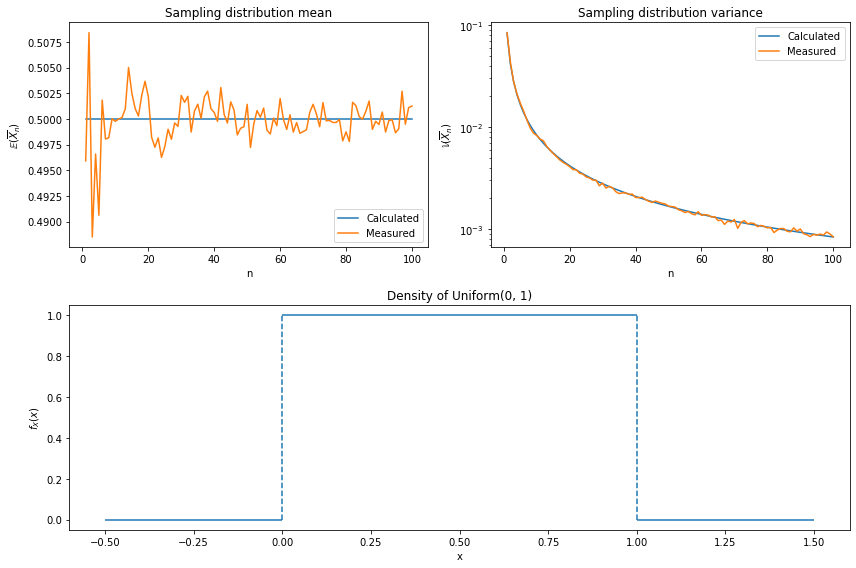
\includegraphics{Figure-04-03}
\end{figure}

Calculated and simulated values agree.

\textbf{Exercise 4.17.20}. Prove Lemma 4.20.
If \(a\) is a vector and \(X\) is a random vector with mean \(\mu\) and
variance \(\Sigma\) then
\[
\EXP(a^T X) = a^T \mu
\quad \text{and} \quad
\VAR(a^T X) = a^T \Sigma a
\]
If \(A\) is a matrix then
\[
\EXP(A X) = A \mu
\quad \text{and} \quad
\VAR(AX) = A \Sigma A^T
\]

\textbf{Solution}.
We have:
\[
\EXP(a^T X) = \begin{pmatrix}
\EXP(a_{1} X_{1}) \\
\EXP(a_{2} X_{2}) \\
\cdots \\
\EXP(a_{k} X_{k})
\end{pmatrix} = \begin{pmatrix}
a_{1} \EXP(X_{1}) \\
\EXP(X_{2}) \\
\cdots \\
\EXP(X_{k})
\end{pmatrix} = a^T \mu
\]
and
\[
\VAR(a^T X) = \EXP((a^T (X - \mu) (a^T(X - \mu))^T) = \EXP((a^T (X - \mu) (X - \mu)^T a) = a^T \Sigma a
\]
Similarly, for the matrix case,
\[
\EXP(AX) = \begin{pmatrix}
\EXP\left( \sum_{j=1}^{k} a_{1, j} X_{j} \right) \\
\EXP\left( \sum_{j=1}^{k} a_{2, j} X_{j} \right) \\
\cdots \\
\EXP\left( \sum_{j=1}^{k} a_{k, j} X_{j} \right) \\
\end{pmatrix} = \begin{pmatrix}
\sum_{j=1}^{k} a_{1, j} \EXP(X_{j}) \\
\sum_{j=1}^{k} a_{2, j} \EXP(X_{j}) \\
\cdots \\
\sum_{j=1}^{k} a_{k, j} \EXP(X_{j}) \\
\end{pmatrix} = A \mu
\]
and
\[
\VAR(A X) = \EXP((A (X - \mu) (A(X - \mu))^T) = \EXP((A (X - \mu) (X - \mu)^T A^T) = A \Sigma A^T
\]

\textbf{Exercise 4.17.21}. Let \(X\) and \(Y\) be random variables.
Suppose that \(\EXP(Y|X) = X\). Show that
Cov\((Y, X) = \VAR(X)\).

\textbf{Solution}. We know that \[
Cov(X, Y)
\]
\[
= \EXP(X \cdot Y) - \EXP(X) \cdot \EXP(Y)
\]
\[
= \EXP(X \cdot Y) - \EXP(X) \cdot \EXP(\EXP(Y|X))
\]
\[
= \EXP(X\cdot Y) - \EXP(X) \cdot \EXP(X)
\]
Hence we only need to show that
\[
\EXP(X\cdot Y) = \EXP(X \cdot \EXP(Y|X))
\]
This is true, since \(E(Y) = EE(Y|X)\). Therefore \[
Cov(X, Y)
\]
\[
= \EXP(X\cdot Y) -  \EXP(X) \cdot \EXP(X)
\]
\[
= \EXP(X \cdot \EXP(Y|X)) -  \EXP(X) \cdot \EXP(X)
\]
\[
= \EXP(X\cdot X) -  \EXP(X) \cdot \EXP(X)
\]
\[
= Cov(X, X)
\] \[
= V(X)
\]
